% Created by tikzDevice version 0.12.3.1 on 2022-01-16 03:38:13
% !TEX encoding = UTF-8 Unicode
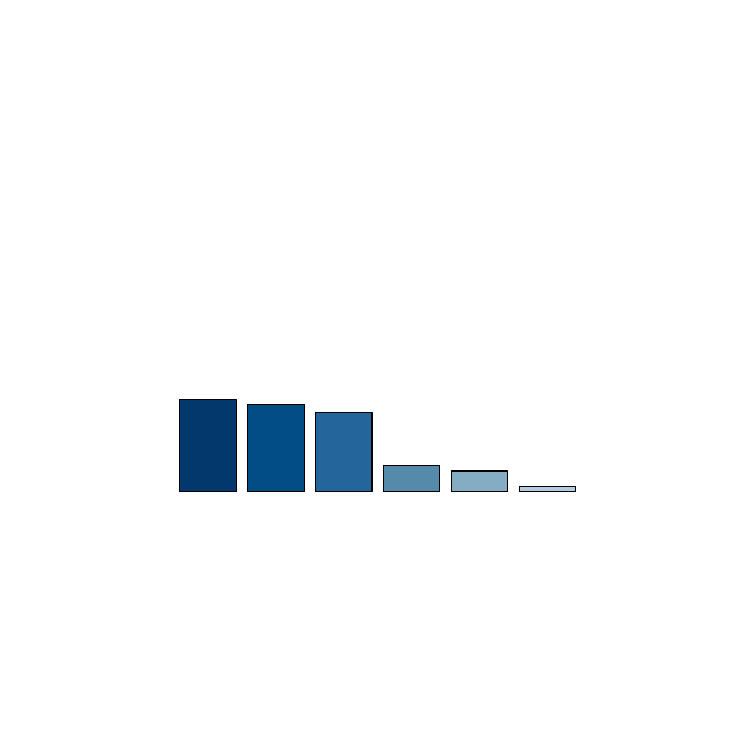
\begin{tikzpicture}[x=1pt,y=1pt]
\definecolor{fillColor}{RGB}{255,255,255}
\path[use as bounding box,fill=fillColor,fill opacity=0.00] (0,0) rectangle (252.94,252.94);
\begin{scope}
\path[clip] (  0.00,  0.00) rectangle (252.94,252.94);
\definecolor{drawColor}{RGB}{0,0,0}
\definecolor{fillColor}{RGB}{2,57,108}

\path[draw=drawColor,line width= 0.4pt,line join=round,line cap=round,fill=fillColor] ( 54.92, 85.20) rectangle ( 75.37,118.73);
\definecolor{fillColor}{RGB}{2,77,132}

\path[draw=drawColor,line width= 0.4pt,line join=round,line cap=round,fill=fillColor] ( 79.45, 85.20) rectangle ( 99.90,116.68);
\definecolor{fillColor}{RGB}{36,102,155}

\path[draw=drawColor,line width= 0.4pt,line join=round,line cap=round,fill=fillColor] (103.99, 85.20) rectangle (124.43,113.94);
\definecolor{fillColor}{RGB}{86,138,171}

\path[draw=drawColor,line width= 0.4pt,line join=round,line cap=round,fill=fillColor] (128.52, 85.20) rectangle (148.96, 94.78);
\definecolor{fillColor}{RGB}{132,172,195}

\path[draw=drawColor,line width= 0.4pt,line join=round,line cap=round,fill=fillColor] (153.05, 85.20) rectangle (173.49, 92.73);
\definecolor{fillColor}{RGB}{178,204,223}

\path[draw=drawColor,line width= 0.4pt,line join=round,line cap=round,fill=fillColor] (177.58, 85.20) rectangle (198.02, 87.25);
\end{scope}
\end{tikzpicture}
